\chapter{Preliminary analysis}


This chapter will analyse existing tools and programming languages that can be used to introduce young people to programming, as well as the fundamentals of game development, to better understand how to design a new programming language that can assist in introducing and engage young people to programming and computer science in general. At the end of this chapter, a problem statement will be defined as a basis for the language that will be designed later in this report.

\section{Beginner friendly programming}
A lot of programming languages can be difficult to use for children and users with little to no experience in programming, as they are not used to the large amount of symbols, the logic behind control flow statements, and the even larger amount of keywords.

This chapter will therefore examine some of the characteristics that are needed for a language to be beginner friendly, both in terms of language design, but also in terms of what kind of, if any, Integrated Development Environment (IDE) should be provided with the language compiler.
An obvious example of an easy-to-learn for beginners language could be Scratch\cite{scratch}, which has an online IDE and compiler on one page. A great part of the success of Scratch comes from exactly that - the integrated IDE/compiler - which is incredibly easy for a kid to use.
Some widely used programming languages are not as beginner friendly as Scratch. Take for example this piece of code in Scheme:
\begin{figure}[H]
    \centering
    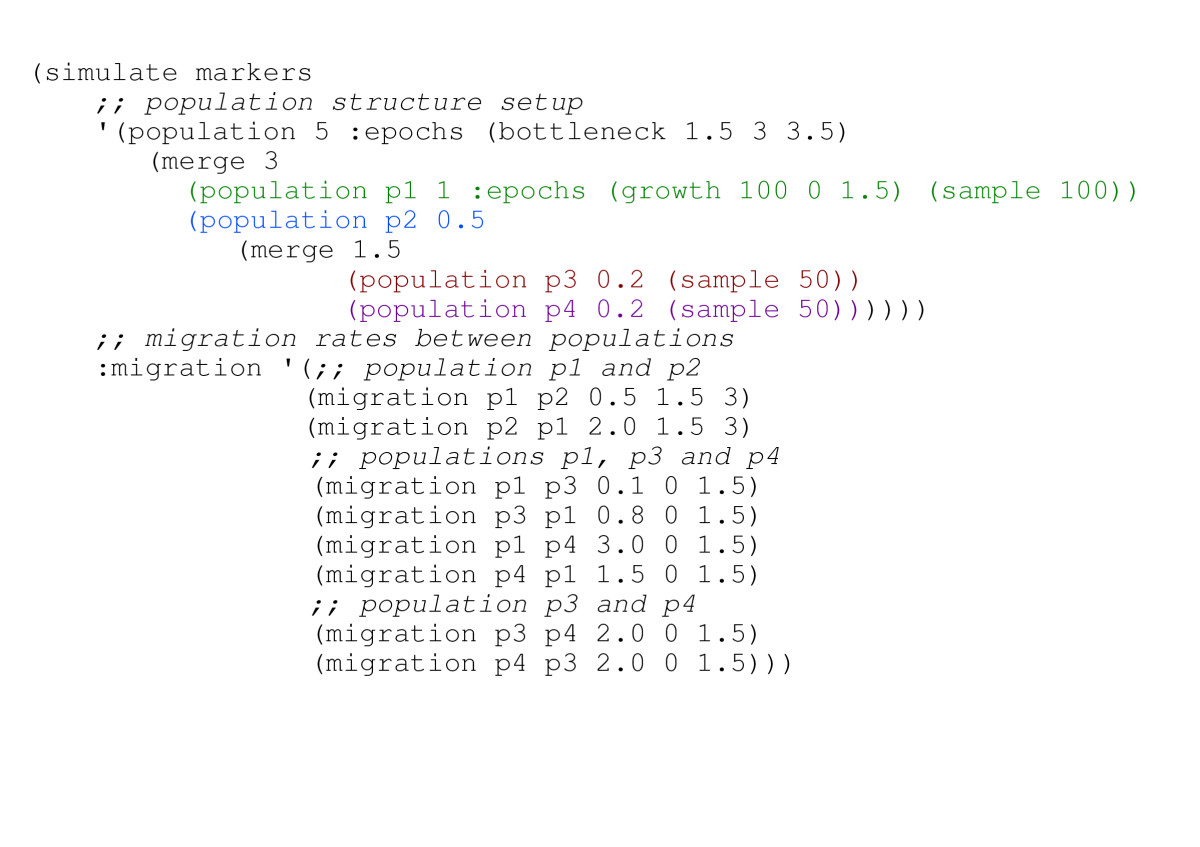
\includegraphics{resources/Images/schemes***.png}
    \caption{This example is supposed to function like a basic for-loop. It does something ten times.}\cite{Schemeexample}\label{fig:schemestuff}
\end{figure}

To the untrained eye, this will seem confusing. The keywords are not inherently easy to understand, and there are numbers/other symbols dispersed all over the code. Furthermore, the amount of parenthesis can easily confuse the user, as it is not clear which parenthesis belongs together, or even why they are there in the first place.

\subsection{Beginner friendly language design}
When making a language beginner friendly, there are a couple of things that should be taken into account. This section talks about the importance of keywords, dynamic and static typing, syntax structure, and type simplicity.
\subsubsection{Keywords}
The meaning (semantics) of a keyword should be readily seen, and intuitive when it is initially looked at. For example, the \textit{namespace} keyword in C\# can be used to declare a scope which can contain a collection of related objects. The objects could for example all belong to the same application, or maybe the same framework. It can be compared to sets in the mathematical fields, which is a collection of related symbols. Namespaces are a very common concept within programming and other computer related fields, but outside that, it is not really widely used or understood. Young users of programming languages will probably not have encountered the word before, and as such, it will contribute to the confusion of learning a new language. If instead of "namespace", something like "scope" or "set" had been used. It would help young users, or users new to programming in general to not be confused when initially learning the language.


\subsubsection{Dynamic and static typing}
Dynamic or static typing is very important for the readability of a language It is therefore important to make the right choice for new users. 
\\Dynamic typing means that a keyword like \textit{var} can be used in C\#, which allows the actual type of a variable to be determined at runtime. This can lead to a lot of confusion when type conversion exceptions are suddenly thrown during execution, because the user realistically has no idea what type of variable actually is in the variable. The upside is that it takes less time to write in this language, as the programmer does not have to think about what type the programmer wants something to be, and what representation of it the programmer wants to use. 
\\Static typing means that the programmer has to use the explicit type they want a variable to be when you are declaring it. This will usually lead to less confusion for inexperienced programmers, as they have to think about what they want a variable to be, and not just remember it based on what they do to that variable. This can however lead to confusing problems when converting between similar types, as for example in c\#, where there are multiple types for number-representation, such as: int, double and decimal. Some conversions between these are allowed, and others are not, which can lead to extra work and confusion when a type suddenly will not fit the input the programmer is giving it.

A language for beginners has to be clear and readable, and this is the main reason that static typing is better for beginners than dynamic typing. If the language is static, the beginner will not have unforeseen conversion errors, or variables that get the wrong input. Of course, cases as the one with multiple representations of numbers in c\# has to be avoided when using static typing. 


\subsubsection{Syntax structure}
When designing a syntax structure that is easy to read for beginners, simplicity is not the main focus, but rather readability. For example in Pascal, all variables has to be declared in the beginning of a function - or procedure as it is called in Pascal:

\lstset{language=[Sharp]C}  
\begin{figure}[H]
\centering
\begin{lstlisting}
procedure DoSomething; 
 var 
  x : Tsome_type;
  y : Tsome_otherType;
  z : Tsome_otherOthertype;
 begin
 if (x > y) then
      z := x
   
   else
      z := x;
   z := z;
 end;
\end{lstlisting}
\caption{Pascal local variable declaration.}\cite{pascalvar}
\label{fig:pascalvar}
\end{figure}
This can lead to somewhat unreadable code, because as it is read, each time a variable is encountered the reader has to go up and look at what kind of variable it is. The upside is that there can never be any doubt about where a variable is declared. A beginner might have a hard time remembering what types all his variables are, and having to go up and look might make it harder to read. 
\\Instead of doing it like in Pascal, it could be done like in Java, which allows variable declaration anywhere:
\lstset{language=[Sharp]C}  
\begin{figure}[H]
\centering
\begin{lstlisting}
public void SomeMethod(){

    int x = 0;
    x = x + 1;
    int y = 100;
    
    public void SomeOtherMethod();
    
    int z = 12;
    x = y+z+x;
    
    public void SomeOtherMethod();
}
\end{lstlisting}
\caption{Pascal local variable declaration.}
\label{fig:javavar}
\end{figure}
This allows variables to be declared where they are needed, and as such, it can improve the readability of the language. The downside of this is that when reading a method, the reader might have to look for a while to find a variable, if it is not properly placed closely to where it is used. 

\subsubsection{Type simplicity}
Keeping the types relatively simple is good for beginners, but only if the meaning of the type is also kept clear. For example, the meaning of \textit{char} in C is relatively clear, but the meaning of something like \textit{struct} is not. \textit{Struct} in itself is rather unintuitive.
So to be usable in a beginner friendly language, types should preferably be kept simple, and without too many different uses. It should not be presumed that beginners inherently know anything about the different constructs in programming. The meaning of a given type needs to be discernible from the type name.
\newpage
\subsection{Beginner friendly tools}
As a beginner, one of the most daunting tasks can be choosing the development environment in which to write code. In some languages, this is taken care of for you. For example in Scratch\cite{scratch}, where the only way to actually "write" in the language is through their website, with a visually based way of defining a program. 
If a beginner was to, for example, start in C\#\cite{CSHARP} and by extension use visual studio, it could be a very confusing experience. Visual studio has a mess of options, toolbars, windows and the like:
\begin{figure}[H]
    \centering
    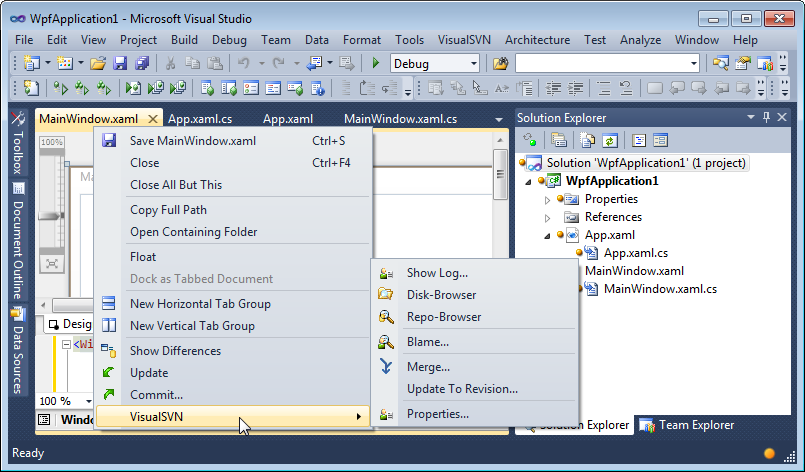
\includegraphics[scale=0.5]{resources/Images/vsclutter.png}
    \caption{Visual Studio clutter}
    \label{fig:vsclutter}
\end{figure}

This is hard to understand without some knowledge of programming beforehand. Therefore, it is useful for a beginner friendly programming language to have some kind of user friendly Interactive Development Environment (IDE) to let the user program in. Otherwise, it is going to be difficult for beginners to get started with programming in the language.
To summarize, it is important that the readability of the language is great when designing for beginners and kids. A more verbose syntax should be preferred over a clean and simple one, like in C\#\cite{CSHARP}, to make the writing of the language closer to actually writing a story, rather than programming a computer to do tasks. Types and keywords have to be intuitive in their use, and the complexity of any given type or keyword cannot be too great, or the readability will suffer from it. Furthermore, the medium in which the language is written is important. A user friendly IDE is paramount to help beginners getting started in a beginner friendly language.
\section{Game development}
In this section, the different components of video game development and how it differs from ordinary application development are analysed. Afterwards, some examples of tools for game development are described, namely \textit{Scratch}, GameMaker and PyGame. This is done to develop a better understanding of which kinds of tools are available to a new developer.

%This section will analyse how games are developed right now, how flow of the project is when you program the game and how this flow can different then a more normal project flow, in a company where you have to make program to some one. after this there will be a look at some of the tools that exist to make this easy for people to program like block programing, here should be look at scratch, then there are combination of block and text programing, here should be look at GameMaker since this still have block program but also text base program in the languge GML(GameMaker Language) and at last only text base programing in this case here should be looked at PyGame this is in python and is a layer over SDL that give easy access to some thing that you need in game develoment.

\subsection{Components of game development}
%To better understand how game development differs from more conventional development, it is important to first understand how to develop a video games.


To develop a video game, the developer needs to manage components that are specific for the domain of game development. All video games must be able to handle user input and have a way to display some sort of output to the user. This output is often in the form of graphics drawn by the graphics card to the screen. Depending on the kind of video game that is being developed, different components are needed. These components include, but are not limited to: 

\begin{itemize}
 \item Collision Detection
 \item Physics
 \item Animation
 \item Graphics (2D and 3D)
 \item Artificial Intelligence
 \item User Input
 \item File Input/Output
 \item Networking \ldots
\end{itemize}

%When developers work on a game they work close together with a team of game designers in bigger companies, they stand for the vision of the game, how they think it should what could be fun the sound the image models and all of those tings you job as the game programmer is to take there's vision and turn it in to realty on the hardware and software you have. and this can be very hard since there so many components in the development of a game, a few things you need to make.\cite{DesignVSPrograming2016}

There are different tools and frameworks that add abstraction layers to game development so that a developer can focus on developing a game, instead of having to spend a lot of time on implementing things like graphics, physics and networking. Some of these tools are described in the following section.

%many of those things can be made easy to understand and use in a program language that is design to make games in, and this will give a faster and better work, and can help introducing new people the programing and game development.

%To answer the question "How is the flow of game development different than programming a normal piece of software?",  \cite{StackGameVSSoftware2011} on a forum post there have been a few people that did talk about their experience in the field of gaming, and how they think it is different, one say that the different lay in the size of the project and a bigger risk and other say that it is the target of what you try to do, when you make a program for a company, you need to make it easy to use and have all the features that ask for, but in the game you need besiege the easy of use also that it is fun to use/play, and that have to think about this under the hole project is he say was the hardes part, and they there where those that say that there were no real different between the two that it was the same thing, so like with software you make for other company's it is something that chance from project to project and is never the same.



\subsection{Existing solutions}
There is a number of tools to develop video games. To best understand the domain, three different tools are described in the following section, namely \textit{Scratch}, \textit{GameMaker} and \textit{PyGame}.
These have been chosen, since they each represent a different approach to video game development.

%In this subsection, three different existing tools with three different approaches are described. The first solution uses block programming only, the second uses both block programming and textual programming, and the third uses textual programming only. This way, \todo{pls help}

\subsubsection{Scratch}
Scratch is a visual programming language, which means that the user programs with a graphical interface rather than a textual one. It utilises block programming instead of actual code. This way, the user does not learn to write code, but rather the mindset of programming. The blocks are conveniently grouped in relevant groups. For example, the group "motion" contains the "move" block, which makes the character move a certain amount of steps, and "turn" blocks, which makes the character turn either clockwise or counterclockwise. By putting these kinds of blocks together, Scratch translates it to actual code.

\begin{figure}[H]
\centering
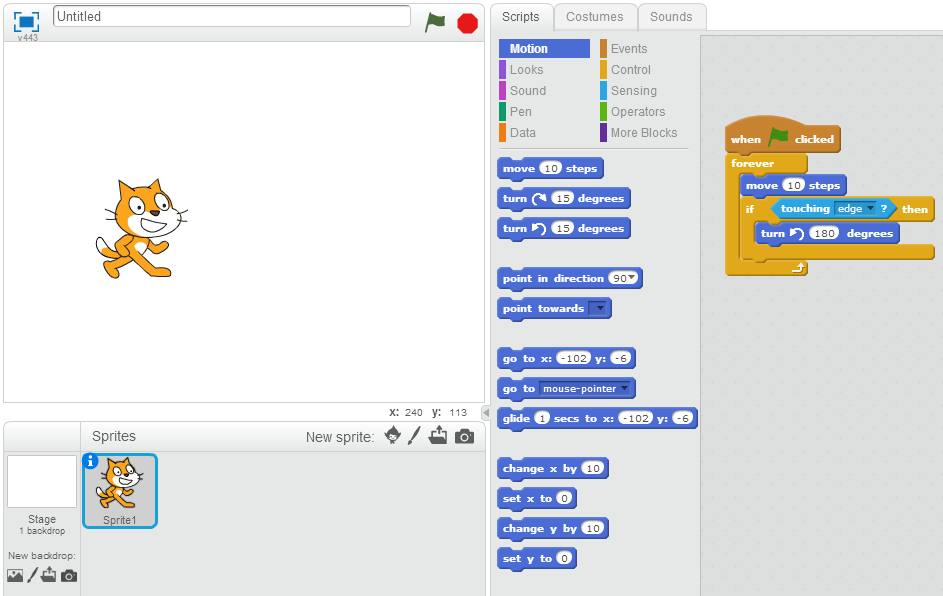
\includegraphics[scale=0.5]{resources/Images/Scratch.png}
\caption{Small program made in Scratch}
\label{fig:Scratch}
\end{figure}

On figure \ref{fig:Scratch} a simple program made in Scratch is seen. This program makes the character indefinitely walk 10 steps in one direction and rotate the character 180 degrees if it hits the wall. The green flag corresponds to running the main function of a conventional programming language.
The easy-to-learn interface and the child friendly design, makes Scratch an ideal solution for the youngest people who wants to be introduced to the world of programming.\cite{scratch}

\subsubsection{GameMaker}
GameMaker is a game making software that implements a mixture of drag and drop programming and their own language called GameMaker Language, which is an interpreted scripting language based on C. This way, it is possible to create games quickly and easily with the drag and drop while at the same time having flexibility and control of conventional programming with GameMaker Language.

\begin{figure}[H]
\centering
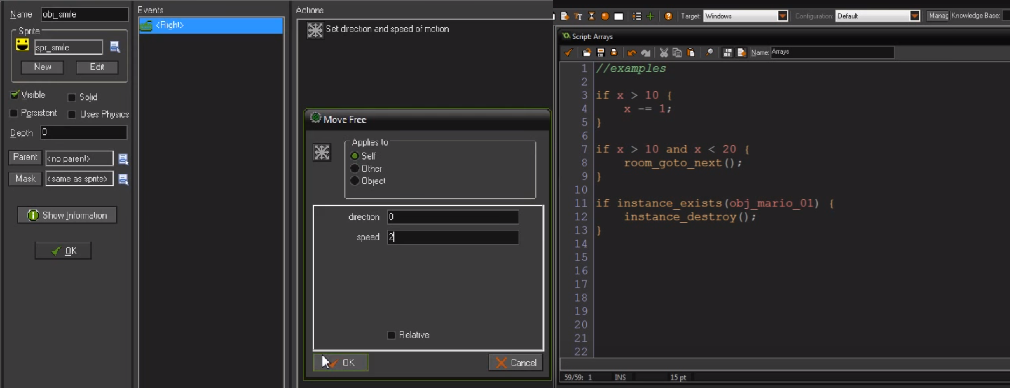
\includegraphics[scale=0.5]{resources/Images/GameMaker.PNG}
\caption{On the left is drag and drop\cite{GMDnD}. On the right is GML \cite{GML}}
\label{fig:GameMaker}
\end{figure}

On figure \ref{fig:GameMaker} an example of the two is shown. On the left is the drag and drop system, where actions gets paired with events. In this example, the right arrow key makes obj\_smile move 2 pixels per frame towards direction 0. On the right side, examples of if-statements in GML are pictured.

\subsubsection{PyGame}
PyGame is a set of Python modules used to make it easier to make games in the programming language Python. This means that it adds a number of functionalities which aid in the game making process. PyGame utilises fully conventional coding and requires the programmer to write actual code.
An example of functionalities is pygame.event.get(), which retrieves every event currently in queue to get handled.

\begin{figure}[H]
\centering
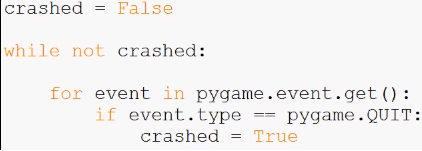
\includegraphics[scale=0.6]{resources/Images/PyGame.png}
\caption{Small PyGame program}
\label{fig:PyGame}
\end{figure}

Figure \ref{fig:PyGame} uses this functionality by checking every event in the queue. Furthermore, it uses pygame.QUIT which is the event type in PyGame that means that the close button has been pressed. Therefore, this code checks every event in the queue if they are a click on the close button. If they are, the program breaks out of the for loop.

\subsection{Target audience}
\label{sub:TargetAudience}
The tools described in this chapter cover a wide spectrum in terms of beginner friendly game development. Scratch\cite{scratch} is easy to use for beginners, and Pygame is meant for more experienced developers. There is, however, a slot somewhere in between Scratch and GameMaker/Pygame, which has to help beginners going from scratch to something like Pygame, and introduce them to control structures, boolean logic, and other concepts of programming. This transition could turn some off from wanting to do more programming, as it may seem too complicated and scary. This is why there is a need for a language in between these two types of programming languages that is simple and easy to learn. Furthermore Scratch looks and feels child-friendly, which is not appealing for a teenager, who wants to be introduced to some less basic concepts of programming while at the same time not getting a lot of advanced and confusing features.

For a textual programming language to have any functionality, it has to use mathematics. These include vectors used in, among others, simulating motion of objects and basic algebra used in variables, which are very essential parts of game development.
As these are an essential part of programming, the target audience has to know, or at least have the preliminary knowledge needed to learn these concepts. As seen in \cite{FFMM} from the Ministry of education, students are introduced to use variables from around the sixth grade in Denmark, but will not learn to use functions and equations before seventh to ninth grade. Therefore, the target audience (TA) is chosen to be students starting from the ninth grade.



With this in mind, there will in the following section be defined a problem statement.
\newpage
\section{Problem statement}
\label{sec:problemstatement}
The goal of this paper is to design and develop a beginner friendly programming language that can help to motivate and introduce young people to programming.

To build upon the knowledge that the end user has about mathematics and logic, as described in \ref{sub:TargetAudience}, and to give them a foothold in the world of programming, some concepts are more appropriate than others, and will therefore be the main focus of the language described in this paper. These concepts are as follows:

\begin{itemize}
    \item Control flow.\\
    This is important for new programmers to understand, since it lies at the root of the most popular programming languages. Having an understanding of control flow, such as if/else constructs can help the user to better understand structured programming.
    
    \item Variables.\\
    As stated in \ref{sub:TargetAudience}, the end user of the language is assumed to have a basic understanding of algebra. This includes simple algebraic problems such as "Find x, when x + 2 = 4". The next natural step, for the user, is to learn about variables, since this may help them to better understand algebra by giving a real life use for it.
    
    \item Object oriented programming.\\
    Having focus on simple object oriented concepts may help the user to understand the mindset of object oriented programming, making it easier to learn a more complex object oriented programming language in the future.
    Furthermore, it is easier to create games with an object oriented language, and it is easier for a beginner to model the program after real life.
    %Having focus on simple object oriented concepts, may help the user to figure out how to write a program, since this can help the user to model the program after what they see in the real world.
\end{itemize}


Since the language described in this paper is designed specifically to aid beginners with developing simple video games, it is advantageous for the language to be domain specific, i.e a domain-specific language (DSL). This way, the end user can focus on developing and designing games instead of worrying about drawing graphics and other technical problems in game design. To attain this, the language should implement common constructs used in game design to apply abstraction layers to the technical part of developing a video game.

From all this, and based on the rest of the analysis, the following problem statement has been defined:

\textit{How can a domain-specific language that can help to motivate and introduce young people to programming, in particular to concepts like control flow, variables and other basic concepts from object oriented programming, be designed and developed, such that the end user can focus on designing and implementing simple games and not worry about the more technical part of game development?}








